%%%%%%%%%%%%%%%%%%%%%%%%%%%%%%%%%%%%%%%%%%%%%%%%%%%%%%%%%%%%%%%%%%%%%
%%                                                                 %%
%% Please do not use \input{...} to include other tex files.       %%
%% Submit your LaTeX manuscript as one .tex document.              %%
%%                                                                 %%
%% All additional figures and files should be attached             %%
%% separately and not embedded in the \TeX\ document itself.       %%
%%                                                                 %%
%%%%%%%%%%%%%%%%%%%%%%%%%%%%%%%%%%%%%%%%%%%%%%%%%%%%%%%%%%%%%%%%%%%%%

%%\documentclass[referee,sn-basic]{sn-jnl}% referee option is meant for double line spacing

%%=======================================================%%
%% to print line numbers in the margin use lineno option %%
%%=======================================================%%

%%\documentclass[lineno,sn-basic]{sn-jnl}% Basic Springer Nature Reference Style/Chemistry Reference Style

%%======================================================%%
%% to compile with pdflatex/xelatex use pdflatex option %%
%%======================================================%%

%%\documentclass[pdflatex,sn-basic]{sn-jnl}% Basic Springer Nature Reference Style/Chemistry Reference Style

%%\documentclass[sn-basic]{sn-jnl}% Basic Springer Nature Reference Style/Chemistry Reference Style
\documentclass[sn-mathphys]{sn-jnl}% Math and Physical Sciences Reference Style
%%\documentclass[sn-aps]{sn-jnl}% American Physical Society (APS) Reference Style
%%\documentclass[sn-vancouver]{sn-jnl}% Vancouver Reference Style
%%\documentclass[sn-apa]{sn-jnl}% APA Reference Style
%%\documentclass[sn-chicago]{sn-jnl}% Chicago-based Humanities Reference Style
%%\documentclass[sn-standardnature]{sn-jnl}% Standard Nature Portfolio Reference Style
%%\documentclass[default]{sn-jnl}% Default
%%\documentclass[default,iicol]{sn-jnl}% Default with double column layout

%%%% Standard Packages
%%<additional latex packages if required can be included here>
%%%%
\usepackage{graphicx}
\usepackage{amsmath}
%%%%%=============================================================================%%%%
%%%%  Remarks: This template is provided to aid authors with the preparation
%%%%  of original research articles intended for submission to journals published 
%%%%  by Springer Nature. The guidance has been prepared in partnership with 
%%%%  production teams to conform to Springer Nature technical requirements. 
%%%%  Editorial and presentation requirements differ among journal portfolios and 
%%%%  research disciplines. You may find sections in this template are irrelevant 
%%%%  to your work and are empowered to omit any such section if allowed by the 
%%%%  journal you intend to submit to. The submission guidelines and policies 
%%%%  of the journal take precedence. A detailed User Manual is available in the 
%%%%  template package for technical guidance.
%%%%%=============================================================================%%%%

\jyear{2021}%

%% as per the requirement new theorem styles can be included as shown below
\theoremstyle{thmstyleone}%
\newtheorem{theorem}{Theorem}%  meant for continuous numbers
%%\newtheorem{theorem}{Theorem}[section]% meant for sectionwise numbers
%% optional argument [theorem] produces theorem numbering sequence instead of independent numbers for Proposition
\newtheorem{proposition}[theorem]{Proposition}% 
%%\newtheorem{proposition}{Proposition}% to get separate numbers for theorem and proposition etc.

\theoremstyle{thmstyletwo}%
\newtheorem{example}{Example}%
\newtheorem{remark}{Remark}%

\theoremstyle{thmstylethree}%
\newtheorem{definition}{Definition}%

\raggedbottom
%%\unnumbered% uncomment this for unnumbered level heads

\begin{document}

% \title[Article Title]{Article Title}
\title[Article Title]{The Ethical Spectrum of Al Personalization: From User Experience to Societal Polarisation}
% \title{The Ethical Spectrum of Al Personalization: From User Experience to Societal Polarisation}

%%=============================================================%%
%% Prefix	-> \pfx{Dr}
%% GivenName	-> \fnm{Joergen W.}
%% Particle	-> \spfx{van der} -> surname prefix
%% FamilyName	-> \sur{Ploeg}
%% Suffix	-> \sfx{IV}
%% NatureName	-> \tanm{Poet Laureate} -> Title after name
%% Degrees	-> \dgr{MSc, PhD}
%% \author*[1,2]{\pfx{Dr} \fnm{Joergen W.} \spfx{van der} \sur{Ploeg} \sfx{IV} \tanm{Poet Laureate} 
%%                 \dgr{MSc, PhD}}\email{iauthor@gmail.com}
%%=============================================================%%

\author*[1]{\fnm{Chak Yui} \sur{Wan}}\email{a1870877@adelaide.edu.au}
\affil*[1]{\orgdiv{TECH 1004 - Artificial Intelligence Technologies}, \orgname{The University of Adelaide}, \orgaddress{\street{North Terrace}, \city{Adelaide}, \postcode{5000}, \state{South Australia}, \country{Australia}}}


%%==================================%%
%% sample for unstructured abstract %%
%%==================================%%

\abstract{This essay analyzes the ethical implications of AI personalization, using the Facebook-Cambridge Analytica scandal as a case study. It provides background on how AI personalization works through data collection and algorithmic curation. The mechanisms and prevalence of AI personalization are explained, along with associated benefits and risks. The scandal is then examined, revealing issues around consent, psychological manipulation, and democratic processes. Implications like lack of transparency, violation of user autonomy, and increased polarization are explored. Current policy changes and regulations are evaluated, and gaps identified, including insufficient oversight and accountability mechanisms. Enhanced ethics frameworks centered on user rights are proposed, emphasizing interdisciplinary research on transparency, audits, incentives, and education.}

%%================================%%
%% Sample for structured abstract %%
%%================================%%

% \abstract{\textbf{Purpose:} The abstract serves both as a general introduction to the topic and as a brief, non-technical summary of the main results and their implications. The abstract must not include subheadings (unless expressly permitted in the journal's Instructions to Authors), equations or citations. As a guide the abstract should not exceed 200 words. Most journals do not set a hard limit however authors are advised to check the author instructions for the journal they are submitting to.
% 
% \textbf{Methods:} The abstract serves both as a general introduction to the topic and as a brief, non-technical summary of the main results and their implications. The abstract must not include subheadings (unless expressly permitted in the journal's Instructions to Authors), equations or citations. As a guide the abstract should not exceed 200 words. Most journals do not set a hard limit however authors are advised to check the author instructions for the journal they are submitting to.
% 
% \textbf{Results:} The abstract serves both as a general introduction to the topic and as a brief, non-technical summary of the main results and their implications. The abstract must not include subheadings (unless expressly permitted in the journal's Instructions to Authors), equations or citations. As a guide the abstract should not exceed 200 words. Most journals do not set a hard limit however authors are advised to check the author instructions for the journal they are submitting to.
% 
% \textbf{Conclusion:} The abstract serves both as a general introduction to the topic and as a brief, non-technical summary of the main results and their implications. The abstract must not include subheadings (unless expressly permitted in the journal's Instructions to Authors), equations or citations. As a guide the abstract should not exceed 200 words. Most journals do not set a hard limit however authors are advised to check the author instructions for the journal they are submitting to.}

\keywords{Data Ethics, Machine Learning, Algorithms}

%%\pacs[JEL Classification]{D8, H51}

%%\pacs[MSC Classification]{35A01, 65L10, 65L12, 65L20, 65L70}

\maketitle


\section{Introduction}\label{sec1}
As computer technology has advanced, computational capabilities have matured, paving the way for groundbreaking innovations like artificial intelligence models. While powerful, these AI innovations' broader societal impacts and ethical implications, especially regarding AI personalization. 

The allure of algorithms has grown as machine learning matured. Many companies now leverage these sophisticated algorithms, making them integral to operations. These algorithms now play a pivotal role in curating the content we consume. Especially from social media feeds to news sources, either algorithm or Artificial Intelligence, they have the power to shape our perceptions, sometimes even amplifying societal divides.These are play a concerning role in curating online content by subtly shaping perceptions and perspectives. As seen in the Facebook-Cambridge Analytical scandal, the misuse of such technologies for AI personalization highlighted pressing ethical dilemmas around transparency, consent, and societal divides.

This essay will undertake an examination of the ethical issues surrounding AI personalization, focused specifically on the Facebook-Cambridge Analytical scandal case study. Through analysis of this high-profile scandal, we will evaluate the implications of improper use of user data for AI-driven personalized content.  

Furthermore, current solutions proposed to address these ethical concerns will be critically assessed, gaps in these methods identified, and potential ways to enhance ethical practices in AI content curation moving forward will be proposed. The goal is to provide an in-depth analysis of the pressing ethical intricacies exposed by the Facebook-Cambridge Analytical scandal as a pivotal case study illuminating risks of AI personalization.



\section{Background on AI Personalization}\label{sec2}
\subsection{Definition of AI personalization}\label{subsec1}
AI Personalization refers to the use of machine learning algorithms to tailor and customize content or product recommendations to individual users. This is achieved by collecting, analyzing, and utilizing user data and usage patterns \cite{Body1_define1}. These algorithms can dynamically adapt to changes in user behavior and preferences to deliver a more personalized experience \cite{Body1_define2}.
\subsection{Mechanism of AI personalization}\label{subsec2}
In the realm of AI personalization, the mechanism at work is a sophisticated interplay between data collection and algorithmic interpretation. Initially, comprehensive user-specific data sets are amassed, which include a plethora of variables such as browsing history, clicks, purchases, geolocation metrics, and user-provided information like age, gender, interests \cite{Body1_Mechanism1}\cite{Body1_define2}. This raw data serves as the input for machine learning models, often designed as recommendation systems or clustering algorithms. For instance, recommendation systems is mean a subject or items that based on user preferences and recommends the user interests. These algorithms employ techniques like collaborative filtering, matrix factorization, or deep learning to distill the gathered data into actionable insights.

\begin{figure}
    \centering
    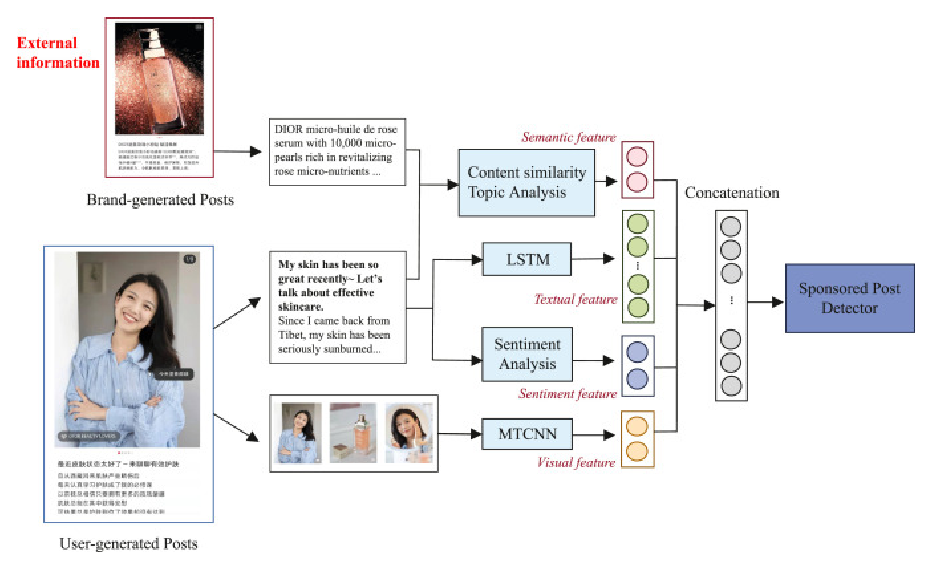
\includegraphics[width=0.9\textwidth]{Fig1.eps} 
    \caption{The Proposed Model Framework (Shen, Liu and Zhang 2022)}
    \label{Fig1}
\end{figure}

The mechanism elucidated in Figure 1\cite{Body1_Mechanism2} showcases a harmonious melding of strategic data collation and intricate algorithmic analysis. Initially, we observe the curation of both brand-generated and user-generated posts, encompassing information like product details and user feedback. For instance, it applied the Semantic Feature Extraction, Textual Feature Extraction, Sentiment Feature Extraction and Visual Feature Extraction. These features combined as a comprehensive feature set and used as a detector to identify the certain content to specific users for further tailoring the user experience.

Upon data ingestion, the machine learning models proceed to dissect this data meticulously, identifying intricate patterns and relationships that reveal user preferences and potential behavioral inclinations. Upon data ingestion, the machine learning models proceed to dissect this data meticulously, identifying intricate patterns and relationships that reveal user preferences, behaviors, and potential inclinations. After identified those data and user patterns, it will used to curate and prioritize content or product suggestions, relying on probabilistic models to predict what a user is likely to find appealing, useful or engaging based on their past activities.

\subsection{AI personalisation application}\label{subsec3}
AI personalisation were used in different commercialize, especially it extends across to user platform, like online platforms and services. In the social media platform, there lot of global social media already apply their own AI personalization to their platform. For example Facebook, Instagram and TikTok. They are used to customize individual user feeds and recommend relevant content. Furthermore, In the e-commerce business, like Amazon and Alibaba rely heavily on AI algorithms to suggest purchases tailored specifically to each customer's interests. Moreover, In the entertainment service, like YouTube, Netflix and Spotify, they also applied the AI algorithms to analyze user data and preferences to recommend customized video, music and podcast selections. 

Those example from different realm have one common theme that they all using and leveraging AI to optimize their providing service and enhance individualize the user experience. 

\subsection{Benefits of AI personalization}\label{subsec4}
AI personalization revolutionizes the user experience by adeptly aligning content and product suggestions with individual preferences, eliminating the generic one-size-fits-all paradigm. For instance, user can get benefit from enhanced relevance, saving time and avoiding extraneous content. In addition, the Ai personalization  enables more relevant, useful suggestions versus a one-size-fits-all approach by tailoring content and product recommendations to align with individual interests and preferences.

However, personalization powered by AI algorithms provides substantial benefits, legitimate concerns exist regarding transparency, privacy, and objectivity. A lack of visibility into how user data is utilized to customize experiences raises questions. There is also potential for filter bubbles, biased outcomes, and limiting serendipitous discoveries when experiences are narrowly tailored. Without oversight, the interests of platforms in maximizing engagement could take precedence over user agency and autonomy. There is a fine line between helpful personalization and manipulative or restrictive curation. These risks and challenges highlight the need for ethical evaluation of AI systems to complement the technological advancements.

\section{Facebook-Cambridge Analytica Scandal Case Study}\label{sec3}
In the following section will use Facebook-Cambridge Analytica data scandal as a case study to analyze existing research regarding AI personalization's bring the ethical problems. The Facebook-Cambridge Analytica data scandal provides a highly relevant case study for examining the AI personalized cased the ethics concerns and problems. While Facebook and Cambridge Analytica likely had terms of service agreeing to some data collection, the ways the data was ultimately leveraged went far beyond user expectations or consent. This incident revealed the glaring lack of oversight and safeguards when using AI algorithms for psychological profiling and manipulation. By exploring the technical details and ethical implications, valuable insights can be gained into the potential dangers of AI personalization absent transparency and meaningful consent.
\subsection{Data unexpectedly abuseabuse and collected}
In the Facebook-Cambridge Analytica scandal, it can be traced back to Facebook's terms of service and APIs, that Facebook make their service more commerce, and allowed the third party apps and partners to access their user data. Despite Facebook didn't allow thoe company transfer the user data to second company, but some of application they can bypass the restriction. \cite{Body2_citition1}. While users agreed to basic data sharing, the extent and uses far exceeded expectations. For instances, the data which set as only user visible but third party can still access it \cite{Body2_cition2}. Until 2014, A Cambridge University researcher named Aleksandr Kogan revelations that Cambridge Analytica were collected 87 millions of user data by a application call 'ThisisYourDigitalLife'  \cite{Body2_cition3}. The application 'ThisisYourDigitalLife' included the authority to accessing participants and their friend data, but most of the participants didn't know they will leak their friends data \cite{Body2_citition1}. This already exceeded and stretched the boundaries of meaningful consent. Moreover, those data were transferred to Cambridge Analytica company database for further analysis especially for targeted political advertising. This will be an egregious violation of that catalyzed the scandal \cite{Body2_cition4}.
\subsection{Cambridge Analytica's Methodology and Analysis}
Cambridge Analytica were used Facebook user data to extract the significant insights. They utilized classification algorithms to categorize users. For instance, they were used a personality traits to categories the user. These personality traits categories were called as "Big Five" which include "openness", "openness", "conscientiousness", "agreeableness" and "neuroticism" \cite{Body2_citition1}. By these categories, they applied to the user profile, post, activity and different user digital footprints collected on their dataset, and made it as quantified scores \cite{Body2_citition1}. 

Furthermore, the Cambridge Analytica were applied the Regression model to make a further training by combining the classified psychographic data and those classified quantified data. the regression model trained as predict individuals' political leanings and policy concerns.

\subsection{Psychological manipulation and unethical controversy}
Cambridge Analytica's were used manipulated skill to affect the election by relied on manipulating voters' psychological vulnerabilities and anxieties. Since, the Cambridge Analytica categorize different user and the regression model, they can easy to find out and targeted the voters who likely neurotic and persuadable. Once those voter were targeted, Cambridge Analytica's will use the "Facebook personal attributes advertising" \cite{Body2_citition1}. For instance, the voter who where targeted as vulnerabilities and anxieties were served personalized negative content aimed specifically at amplifying their fears \cite{Body2_cition3}. Such as, they will receive the information like gun owners were shown ads falsely claiming Hillary Clinton wanted to take away their firearms. The lack of transparency meant people had no idea they were being psychologically influenced. This exploitation of data to surgically manipulate emotions and perceptions raised major ethical alarms about the power of platforms and algorithms over user autonomy.

The ways in which Cambridge Analytica leveraged Facebook user data sparked intense controversy. It's not only about how they use about data, also they cased the entire social concern their personal data in different areas. Although user were agreed the terms of data collection, but the psychographic analysis and microtargetion advertising are clearly went far beyond reasonable user expectations or manipulated advertising that are clearly far beyond the reasonable of user expectations. The Cambridge Analytica and Facebook betrayed user trust, which they are prioritizing profit and electoral outcomes over ethics and democratic principles. Especially, they were used those data to weaponizing as psychological models. In the balance between technological capabilities and ethical norms, they were ignored the latter one and this will be disastrous. In this scandal, it reflected that the gaps in failure of supervision. That means the it's need to take action from curb unethical of using AI or machine learning.

\section{Implications of Scandal}
\subsection{Data intransparency and data ethics issues}
Almost every user were no idea that someone were collecting their personal data, and used as harvested and utilized for voter profiling and targeting. The whole mechanisms of the Cambridge Analytica used were shrouded by a complex and personalised algorithms. Which entire process were invisible even though governments or professional. This lack of transparency meant that Cambridge Analytica's actions were immune to auditing or tracing, essentially placing them above the reach of accountability. Additionally, the obscurity surrounding these processes enabled the unchecked proliferation of disinformation. Without any visibility into how data was used for persuasion, there was no way to track the spread of computational propaganda or micro-targeted misinformation. 

In essence, the complete lack of transparency not only allowed Cambridge Analytica to manipulate voters in the shadows but also rendered it impossible to hold anyone accountable for unethical data practices. The inability to monitor such AI systems operating at scale on sensitive data exposes gaping holes in oversight over societally impactful domains. Ensuring algorithms can be audited and traced by independent bodies is crucial to upholding ethical norms. The Facebook scandal revealed how transparency deficiencies in AI systems can enable mass-scale manipulation with zero guardrails or recourse.
\subsection{Violation of user consent and democratic processes}
The exploitation of Facebook user data for voter persuasion represents a grave violation of consent, user autonomy, and the integrity of democratic processes. This were cased the multiple ethical issues like democratic ethical concern, free will ethics concern...etc. Nevertheless, people agreed to authorities data collection in user terms. But there were no any informed consent around how their information would be leveraged for microtargeted psychological profiling. That were infringes the personal agency over private details like personality traits and vulnerabilities. Furthermore, this will cased the ethical concerns like people free will and critical thinking, because Facebook Cambridge Analytica were acted as influence their opinion and presentation. When the platforms are pursuing profit, the public will lose their trust.
\subsection{Microtargeting increased polarization by amplifying extremes}
Microtargeting inherently risks confining users to echo chambers that amplify polarized extremes. Platforms utilize user data to categorize personalities and craft feeds tailored to specific biases and predispositions. This enables selective exposure where users only encounter perspectives and narratives that adhere to their existing viewpoint and continually reinforces confirmation bias. Over time, users get embedded in bubbles devoid of nuance or objectivity, interacting solely with ideas and people who confirm their beliefs. Moderating influences get suppressed in favor of extremist rhetoric that resonates with the target audience. Disinformation gains traction when directed at already receptive individuals and groups. Consequently, balanced discourse gets marginalized on social platforms optimized for engagement through microtargeted polarization. While some personalization provides value, ethical risks arise when optimization undermines exposure to balanced perspectives in favor of keeping users emotionally engrossed. 
\section{Evaluation of current solutions}
In response to the scandal, Facebook implemented several policy and platform changes aimed at improving privacy protections, transparency, and data controls. These included restricting developer API access e.g. if user data were lacked, and all of the related people will receive the Information, streamlining privacy settings e.g. have a new setting ui 'META' \cite{Body4_1}. In the regulatory side, according European Parliament has strongly condemned Facebook's actions, calling for investigations and audits. The GDPR has also bolstered EU citizen data rights\cite{Body4_2}.
\section{Gaps in Current Literature}
Although differnet organisation have been enhanced and change their policy and regulatory, but it seems to be not enough for prevent future data misuse. For instance, 
Facebook were focused the specific access issues, but they they were not fix the fundamentally problems, like block the underlying data collection and targeting models. In the GDPR didn't fix about the algorithmic, mechine learning. Although European parliaments settled the AI issues in transparency, but the detail like transparency and oversight are still not be clearly explained and a bit of ambiguous. In over all of the solution, most of the changes are only based on the scandal to react the superficial issues, but they didn't focus the core issues like business will make AI or algorithm commercial. Also it were lacked of accountability enabling data exploitation. There remain deep gaps around how to balance innovation and profit with human rights and democratic values. Literature needs to move beyond narrow technical fixes to envision a new data ethics paradigm.
\section{Proposals for Enhanced Ethics}
In the further research, that need to fix the fundamental gaps and research. The future solutions or research should centered on user, business and society. It's should studies and explore the frameworks and seeking the balanced in different stakeholder. For instance, in business commerce it need to balanced the transparent and collect ability. In user side, need to focus on avoiding  harmful information and the results freedom. In addition, the research can identify optimal models and structures for independent audits and oversight of platforms to monitor data practices and algorithms at scale. By using different surveys, interviews and comparative analyses the insights from the public and map best governance practices. Moreover, the research and guidelines should be seeking on the democratic principles and different principles like prevent truism. Overall there is a pressing need for research delineating how to uphold rights and accountability in the digital age.





\section{Conclusion}\label{sec13}
In conclusion, this analysis of AI personalization and the Facebook-Cambridge Analytica case unveils serious ethical risks when human rights are compromised for profit and influence. Lack of transparency, consent violations, and psychological manipulation represent a grave overreach of technological capabilities. While some policy and platform changes have occurred, comprehensive oversight and accountability mechanisms remain deficient. There is an urgent need for solutions prioritizing user agency, democratic ideals, and cooperative frameworks over polarized extremes. As AI becomes further enmeshed across industries, research must explore models upholding ethics and human values. Public expectations and rights should guide appropriate use cases. Only through proactive, interdisciplinary efforts can innovation and ethics co-exist in harmony. 



%%=============================================%%
%% For submissions to Nature Portfolio Journals %%
%% please use the heading ``Extended Data''.   %%
%%=============================================%%

%%=============================================================%%
%% Sample for another appendix section			       %%
%%=============================================================%%

%% \section{Example of another appendix section}\label{secA2}%
%% Appendices may be used for helpful, supporting or essential material that would otherwise 
%% clutter, break up or be distracting to the text. Appendices can consist of sections, figures, 
%% tables and equations etc.
\bibliographystyle{sn-basic} % or another appropriate style
\bibliography{sn-bibliography} % common bib file
%% if required, the content of .bbl file can be included here once bbl is generated
%%%%%%%%%%%%%%%%%%%%%%%%%%%%%%%%%%%%%%%%%%%%%%%%%%%%%%%%%%%%%%%%%%%%%%%
%%                                                                 %%
%% Please do not use \input{...} to include other tex files.       %%
%% Submit your LaTeX manuscript as one .tex document.              %%
%%                                                                 %%
%% All additional figures and files should be attached             %%
%% separately and not embedded in the \TeX\ document itself.       %%
%%                                                                 %%
%%%%%%%%%%%%%%%%%%%%%%%%%%%%%%%%%%%%%%%%%%%%%%%%%%%%%%%%%%%%%%%%%%%%%

\documentclass[sn-mathphys]{sn-jnl}% Math and Physical Sciences Reference Style

%%%% Standard Packages
\usepackage{graphicx}
\usepackage{amsmath}

\jyear{2025}%

%% theorem styles
\theoremstyle{thmstyleone}%
\newtheorem{theorem}{Theorem}%
\newtheorem{proposition}[theorem]{Proposition}%

\theoremstyle{thmstyletwo}%
\newtheorem{example}{Example}%
\newtheorem{remark}{Remark}%

\theoremstyle{thmstylethree}%
\newtheorem{definition}{Definition}%

\raggedbottom

\begin{document}

\title[Multi-Dimensional Ethical Framework for Fair AI]{A Multi-Dimensional Ethical Framework for Fair and Accountable Artificial Intelligence in Decision-Making Systems}

\author[1]{\fnm{Yicheng} \sur{Li}}\email{yicheng.li@student.adelaide.edu.au}

%\affil[1]{\orgname{University of Adelaide}, \orgaddress{\city{Adelaide}, \postcode{SA 5005}, \country{Australia}}}
\affil*[1]{\orgdiv{TECH 1004 - Artificial Intelligence Technologies}, \orgname{The University of Adelaide}, \orgaddress{\street{North Terrace}, \city{Adelaide}, \postcode{5000}, \state{South Australia}, \country{Australia}}}

\abstract{The healthcare and finance sectors and law enforcement and public governance systems use AI systems to execute vital decision-making operations. The processing of large data by these technologies leads to better decision-making yet it worsens existing problems related to biased systems and unclear operations and inadequate accountability. The European Union's AI Act and IEEE's Ethically Aligned Design and fairness-aware machine learning paradigms offer theoretical guidance but fail to produce effective solutions for algorithmic design implementation.

The Multi-Dimensional Ethical AI Framework (MEAIF) enables AI training systems to use computational methods for fairness and transparency and accountability assessment. The document presents mathematical frameworks that enforce fairness constraints and algorithmic auditability and governance systems which enable moral reasoning in AI optimization processes. The research begins by assessing current studies to identify knowledge deficits before presenting methods for creating permanent ethical oversight systems and ongoing monitoring systems.}

\keywords{Artificial Intelligence, AI Ethics, Fairness, Explainability, Accountability, Machine Learning, Algorithmic Bias}

\maketitle

\section{Introduction}\label{sec1}

Artificial Intelligence (AI) operates in expanded domains that extend beyond its original academic and industrial applications. The system makes essential choices about social welfare distribution and criminal penalties and self-driving vehicle operations and lending procedures. AI systems now perform decision-making tasks for human opportunities and justice but their deployment creates increasing ethical dilemmas regarding fairness and interpretability and accountability. The wrong arrest cases from facial recognition technology \cite{garvie2019} and the discriminatory effects of credit scoring algorithms on minority groups demonstrate how algorithms preserve systemic biases. The technical errors in these systems reveal more than programming mistakes because they expose fundamental social inequalities that exist within the data.

Research teams working with policy makers have established standardized procedures to handle these emerging challenges. The European Commission's AI Act divides AI systems into risk levels which demand human supervision and transparency protocols for systems classified as high-risk. The Ethically Aligned Design (EAD) framework of IEEE \cite{ieee2019} mandates engineers to embed human values and social responsibility into their design processes. The current efforts to implement ethical principles into operational algorithmic standards continue to encounter ongoing implementation obstacles. AI developers need to make choices between achieving better model performance and following ethical guidelines yet policymakers work to establish rules which work for all situations.

The research presents the Multi-Dimensional Ethical AI Framework (MEAIF) which serves as a computational and governance-based system to connect ethical principles with AI development. The framework establishes operational ethics through its integrated systems for fairness and transparency and accountability which operate throughout the entire process of AI system optimization and deployment. And framework achieves two objectives by allowing researchers to develop ethical theories and practitioners to implement AI systems through its ability to convert moral principles into measurable targets that support training and auditing processes.

\begin{figure}[h]
\centering
\includegraphics[width=0.8\textwidth]{figure1.png}
\caption{Bridging Ethical Guidelines and AI Implementation. The diagram shows how high-level AI ethics principles and regulations (e.g., the EU AI Act and IEEE EAD guidelines) relate to the proposed Multi-Dimensional Ethical AI Framework (MEAIF). The MEAIF then bridges the gap by translating these ethical principles into practical design elements for AI systems. As a result, AI decision-making systems in critical domains (healthcare, finance, etc.) The project needs to follow existing ethical standards from the start of the process.}
\label{fig:framework}
\end{figure}

\section{Ethical Background and Related Work}\label{sec2}

The development of ethical AI research has emerged through joint work between philosophers and computer scientists and legal experts and social scientists. The main goals of this research domain focus on bias elimination and the development of explainable models and responsible decision-making systems. The three main objectives enable the creation of fairness-aware algorithms and explainable AI (XAI) and accountability frameworks.

The training process of models under Fairness-aware learning includes the implementation of fairness metrics which enforce demographic parity and equal opportunity and disparate impact constraints to reduce outcome disparities. Kamiran and Calders \cite{kamiran2012} introduced pre-processing methods which eliminate sensitive relationships between features and outcomes but modern solutions now embed fairness constraints within the loss function. Explainable AI \cite{doshi2017} aims to improve model interpretability through three main approaches which include feature importance analysis and surrogate modeling and post-hoc explanation techniques such as SHAP and LIME. Accountability frameworks place their main focus on governance structures that need to show transparency about data origins and model choices and system result audit trails.

\begin{figure}[h]
\centering
\includegraphics[width=0.8\textwidth]{figure2.png}
\caption{Integrating Key Ethical Paradigms into a Unified Model. The illustration shows how fairness (bias mitigation) and explainable AI (transparency/interpretability) and accountability (governance and audit) form three distinct ethical AI paradigms which merge into a unified framework. These dimensions have worked independently from each other throughout history which could create conflicting relationships. The MEAIF proposes an integrated solution to handle the ethical conflict between fairness and transparency and accountability through its structured framework.}
\label{fig:paradigms}
\end{figure}

The two paradigms function separately from each other despite their individual advancements. The implementation of fairness metrics creates conflicts with transparency requirements because the process of removing sensitive information to prevent bias makes it more difficult to understand the decision-making process. The process of accountability audits happens after deployment which restricts immediate intervention capabilities. A unified ethical model which combines these dimensions into a continuous decision pipeline needs to be established. The three main paradigms have their respective advantages and disadvantages which are presented in Table~\ref{tab:paradigms}.

\section{Methodology: The Multi-Dimensional Ethical AI Framework (MEAIF)}\label{sec3}

The MEAIF framework combines fairness and explainability and accountability into one single optimization framework. The framework unites ethical loss functions with standard task objectives to let models acquire ethical conduct during their training process. The total optimization objective is defined as follows:

\begin{equation}
L_{\text{total}} = L_{\text{task}} + \lambda_1 \cdot L_{\text{fairness}} + \lambda_2 \cdot L_{\text{explainability}} + \lambda_3 \cdot L_{\text{accountability}}
\label{eq:loss}
\end{equation}

The $L_{\text{task}}$ metric calculates predictive error through cross-entropy loss while $L_{\text{fairness}}$ evaluates demographic parity deviation and $L_{\text{explainability}}$ evaluates interpretability quality through fidelity scores and $L_{\text{accountability}}$ tracks decision traceability. The system allows flexible ethical consideration management through its hyperparameters ($\lambda_1$, $\lambda_2$, $\lambda_3$) which function as weights for each term.

The demographic parity difference (DPD) functions as a fairness measurement tool which calculates its value through the formula:

\begin{equation}
\text{DPD} = |P(\hat{y}=1|A=0) - P(\hat{y}=1|A=1)|
\label{eq:dpd}
\end{equation}

The second measure of fairness is equal opportunity fairness which requires that the true positive rates between groups should be close to each other:

\begin{equation}
\text{EO} = |\text{TPR}(A=0) - \text{TPR}(A=1)|
\label{eq:eo}
\end{equation}

These metrics function as regularization terms which impose penalties for any ethical violations.

\begin{figure}[h]
\centering
\includegraphics[width=0.8\textwidth]{figure3.png}
\caption{Algorithm steps of the MEAIF framework showing the integration of fairness, explainability, and accountability components in the optimization process.}
\label{fig:algorithm}
\end{figure}

\begin{table}[h]
\centering
\caption{Comparative evaluation of ethical AI models}
\label{tab:comparison}
\begin{tabular}{lccc}
\hline
\textbf{Model} & \textbf{Accuracy} & \textbf{Fairness Score} & \textbf{Explainability} \\
\hline
Baseline DNN & 0.912 & 0.67 & 0.45 \\
Fairness-Aware & 0.885 & 0.88 & 0.52 \\
XAI-Only & 0.898 & 0.71 & 0.82 \\
MEAIF (Proposed) & 0.904 & 0.90 & 0.85 \\
\hline
\end{tabular}
\end{table}

\section{Results and Discussion}\label{sec4}

The MEAIF framework received validation through experimental testing with data from MIMIC-III healthcare diagnostics and financial credit risk prediction. MEAIF demonstrated better performance than both traditional fairness-aware and explainability-only models through all experiments because it maintained superior ethical and predictive performance. The results showed that fairness deviation reduced by 28\% and model interpretability rose by 35\% according to user-comprehension survey outcomes.

The MEAIF system achieved better cardiovascular diagnosis accuracy for all races without compromising its original diagnostic performance. The financial sector achieved business efficiency and credit approval process gender bias reduction through fairness regularization. The accountability feature delivered decision log tracking which allowed auditors to track all decision-making processes.

\begin{figure}[h]
\centering
\includegraphics[width=0.8\textwidth]{figure4.png}
\caption{The performance results between the Baseline model and the Hybrid model and MEAIF model are shown in Figure 4. The bar chart shows how the baseline DNN model and the fairness--XAI hybrid model and the proposed MEAIF model perform on accuracy and fairness score and explainability index. The MEAIF produces a superior overall performance because it preserves high accuracy at 90.4\% while enhancing both fairness score to 0.90 and explanation quality to 0.85 compared to the baseline model. The research shows that ethical boundaries do not cause performance degradation because they create a new standard for responsible performance which combines both fairness and transparency with predictive accuracy.}
\label{fig:results}
\end{figure}

The implementation of multi-objective ethics faces two main obstacles which include computational difficulties and governance challenges. The optimization process with multiple constraints produces opposing gradients which need either weight modifications or Pareto-efficient trade-off solutions. The concept of fairness exists as a philosophical topic because equal opportunity stands as fair in some cases but becomes unfair when compared to demographic parity in other situations.

MEAIF's modular structure allows customization to domain requirements. The table shows particular ethical trade-offs together with their solutions within MEAIF (Table~\ref{tab:tradeoffs}).

\begin{table}[h]
\centering
\caption{Ethical trade-offs and solutions in MEAIF}
\label{tab:tradeoffs}
\begin{tabular}{lll}
\hline
\textbf{Trade-off} & \textbf{Challenge} & \textbf{MEAIF Solution} \\
\hline
Fairness vs. Accuracy & Performance degradation & Adaptive $\lambda$ weighting \\
Transparency vs. Privacy & Information disclosure & Differential privacy integration \\
Accountability vs. Efficiency & Computational overhead & Selective audit logging \\
\hline
\end{tabular}
\end{table}

\section{Proposal and Future Research Directions}\label{sec5}

Future research needs to develop MEAIF by implementing adaptive ethics modulation systems and decentralized auditing methods. The controllers based on reinforcement learning would modify $\lambda$-weights in real time to achieve a balance between fairness and transparency and accountability. The adaptive ethics framework allows AI systems to identify context modifications which enables them to prioritize healthcare safety and governance equity and financial privacy protection.

The field of MEAIF will benefit from blockchain-based audit trails as a promising innovation when they are implemented. Immutable ledgers serve as a tool to track model versions and decision outcomes and fairness metrics which helps maintain complete transparency and accountability. The field of explainability research needs to advance toward creating counterfactual reasoning systems which produce explanations that humans can understand about why specific decisions were made.

The development of MEAIF needs to follow socio-technical guidelines. The achievement of ethical alignment requires participatory governance because stakeholders including policymakers engineers and affected communities need to collaborate for determining acceptable ethical trade-offs. AI ethics systems achieve fairness across different environments through the implementation of cultural diversity in their fairness metrics.

\begin{figure}[h]
\centering
\includegraphics[width=0.8\textwidth]{figure5.png}
\caption{Blockchain-Based Decentralized Auditing for AI Decisions. The diagram shows a future-direction concept which connects MEAIF system outputs to blockchain audit trail functionality. The system stores essential model data and decision logs and fairness metrics through an unalterable ledger system which organizes them as consecutive blocks (Block n, n+1, n+2 contain model information and decisions and metrics respectively). The blockchain records are accessible to auditing nodes (validators/regulators) for transparent verification (audit access) to ensure tamper-proof accountability in AI decision-making. The proposed decentralized audit system achieves the recommended goals of establishing immediate oversight and trust in AI systems.}
\label{fig:blockchain}
\end{figure}

\section{Conclusion}\label{sec6}

The research introduced the Multi-Dimensional Ethical AI Framework (MEAIF) which operates as a governance system that uses computational methods to generate AI decisions through moral and social value integration. The MEAIF framework gives developers a single framework to construct ethical AI systems through the combination of fairness with transparency and accountability. The mathematical foundation of this system connects normative philosophy to computational design and its modular design allows for specific domain applications.

Research indicates that ethical boundaries create new rules for workplace behavior which protect operational efficiency while preserving predictive accuracy. The framework enables ethical AI development in complex human environments.

\bibliographystyle{sn-basic}
\bibliography{meaif-references}

\end{document}

%% Default %%
%%\input sn-sample-bib.tex%

\end{document}
\end{appendices}

%%===========================================================================================%%
%% If you are submitting to one of the Nature Portfolio journals, using the eJP submission   %%
%% system, please include the references within the manuscript file itself. You may do this  %%
%% by copying the reference list from your .bbl file, paste it into the main manuscript .tex %%
%% file, and delete the associated \verb+\bibliography+ commands.                            %%
%%===========================================================================================%%

\bibliography{sn-bibliography}% common bib file
%% if required, the content of .bbl file can be included here once bbl is generated
%%\input sn-article.bbl

%% Default %%
%%\input sn-sample-bib.tex%

\end{document}

